\section{Algoritmi di triangolazione}
\label{sec:algoritmi_di_triangolazione}

Un problema classico della computer grafica è quello di scomporre un poligono semplice in un insieme di triangoli i cui vertici sono solo quelli del poligono semplice. Per definizione, un poligono semplice è una sequenza ordinata di $n$ punti. I vertici consecutivi sono collegati da un bordo e l'ultimo bordo collega il primo e l'ultimo punto. Ogni vertice condivide esattamente due spigoli. Gli unici punti in cui è consentito l'intersezione degli spigoli sono i vertici. 
\begin{figure}[htbp]
	\centering
	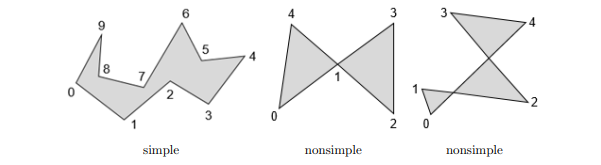
\includegraphics[width=0.75\textwidth]{figures/2_background_teorico/simple-polygon.png}
\end{figure}

La scomposizione di un poligono semplice in triangoli è chiamata triangolazione del poligono.  Qualsiasi triangolazione di un poligono semplice di $n$ vertici ha $n - 2$ triangoli.

Nel corso degli anni sono stati proposti numerosi algoritmi per risolvere il problema della triangolazione di un poligono, che si differenziano tra loro per generalità, complessità computazionale e qualità geometrica dei triangoli prodotti. 
In questa sezione se ne richiamano due tra i più rappresentativi: l'\emph{ear clipping}, il più semplice, e la (\emph{Constrained}) \emph{Delaunay Triangulation}, in grado di produrre triangoli di qualità geometrica superiore.

\subsection{Ear clipping}
\label{subsec:ear_clipping}


L'ear clipping è uno dei metodi più diretti per triangolare un poligono semplice. Il metodo si basa sulla nozione di \emph{orecchio} (\emph{ear}): dati tre vertici consecutivi del poligono, essi formano un orecchio se il vertice centrale è convesso e il segmento che unisce il primo e il terzo vertice è interamente contenuto all'interno del poligono, cioè se il triangolo da essi individuato può essere staccato dal poligono senza uscire dal suo contorno. Un risultato noto in geometria computazionale, il \emph{teorema dei due orecchi}, garantisce che ogni poligono semplice con almeno quattro vertici possieda sempre almeno due orecchi.

Si individua un orecchio, lo si rimuove dal poligono (aggiungendo il triangolo corrispondente all'insieme di output), ottenendo un nuovo poligono, più piccolo, che soddisfa ancora le condizioni del teorema; l'operazione viene ripetuta fino a quando non rimane un solo triangolo.

L'algoritmo è semplice da implementare ma esegue in tempo $O(n^2)$ \cite{eberly2002triangulation}. Esistono varianti più efficienti, come la decomposizione in poligoni monotoni ($O(n \log n)$) o algoritmi randomizzati praticamente lineari, ma sono più complesse da implementare.

\begin{figure}[htbp]
	\centering
	\begin{subfigure}{0.5\textwidth}
		\centering
		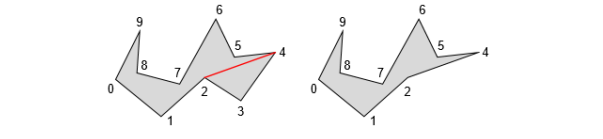
\includegraphics[width=1\linewidth]{figures/2_background_teorico/1-ear-clipping.png}
	\end{subfigure}
	\hfill
	\begin{subfigure}{0.5\textwidth}
		\centering
		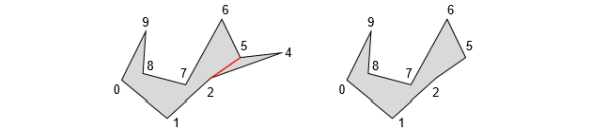
\includegraphics[width=1\linewidth]{figures/2_background_teorico/2-ear-clipping.png}
	\end{subfigure}
	\begin{subfigure}{0.5\textwidth}
		\centering
		
\includegraphics[width=1\linewidth]{figures/2_background_teorico/3-ear-clipping.png}
	\end{subfigure}
	\begin{subfigure}{0.5\textwidth}
		\centering
		
\includegraphics[width=1\linewidth]{figures/2_background_teorico/4-ear-clipping.png}
	\end{subfigure}
	\begin{subfigure}{0.5\textwidth}
		\centering
		
\includegraphics[width=1\linewidth]{figures/2_background_teorico/5-ear-clipping.png}
	\end{subfigure}
\end{figure}


\newpage
\subsection{Triangolazione di Delaunay}
\label{subsec:delaunay_cdt}

Un approccio alternativo, che si applica in generale a un insieme di punti anziché a un poligono, è la triangolazione di Delaunay (\emph{Delaunay Triangulation}, DT): dato un insieme di punti nel piano, la DT suddivide il loro inviluppo convesso in triangoli tali che la circonferenza circoscritta a ciascuno di essi (la circonferenza passante per i suoi tre vertici) non contenga, al proprio interno, nessun altro punto dell'insieme. Questa proprietà ha l'effetto di massimizzare il più piccolo angolo tra tutti i triangoli della triangolazione, evitando così la formazione di triangoli eccessivamente sottili o degeneri (\emph{sliver}).

La DT dipende unicamente dalla posizione dei punti e non tiene conto di eventuali archi che si desidera vedere presenti nella triangolazione risultante: nulla impedisce che un triangolo la "attraversi". La Constrained Delaunay Triangulation (CDT) generalizza la DT introducendo la possibilità di imporre un insieme di segmenti obbligatori (\emph{constraint}), che devono necessariamente comparire come archi della triangolazione finale. L'input al problema della CDT è tipicamente un PSLG: un insieme di punti e di segmenti non incidenti tra loro, questi ultimi trattati come vincoli da rispettare.

Per illustrare questa idea, la figura seguente mostra un esempio di ciò che accade quando un insieme di punti è collegato in modo arbitrario rispetto a uno conforme al criterio di Delaunay \cite{lucas2016delaunay}:
\begin{figure}[htbp]
	\centering
	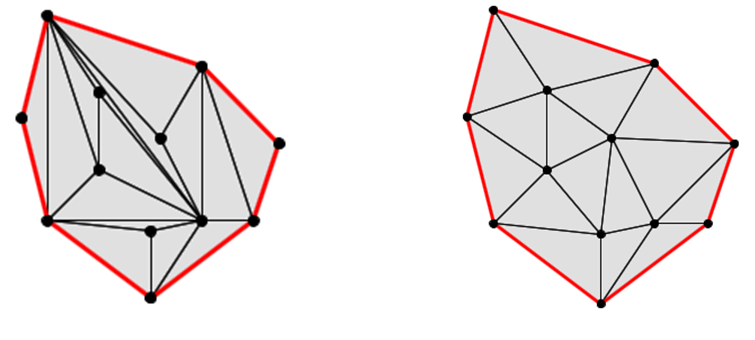
\includegraphics[width=0.5\textwidth]{figures/2_background_teorico/delaunay-triangulation.png}
\end{figure}



Dal punto di vista della complessità computazionale, sono noti diversi algoritmi in grado di calcolare la CDT di un PSLG generico in tempo $O(n \log n)$; nel caso particolare in cui l'input sia un singolo poligono semplice, la CDT può essere calcolata in tempo lineare $O(n)$.

Rispetto all'ear clipping, la CDT presenta due caratteristiche importanti: da un lato tende a produrre triangoli di qualità geometrica superiore evitando la formazione di triangoli degeneri; dall'altro consente di specificare esplicitamente quali segmenti debbano necessariamente far parte della triangolazione risultante.